\chapter{Implementation}
This chapter is concerned with the implementation details of the individidual components introduced in Chapter \ref{chapter:4}. This includes the development of the Unity application responsible for producing the front-facing camera video stream and displaying the visual cues, the development of the human detection and direction system, as well as the reactive control systems implemented on ARTA. Previous work in the PRL had utilized the Hololens camera to capture images that were then processed on an external computer, but where this project differs is that a video stream is required to perform real-time object detection. As such, a large amount of time was spent at the very beginning of the project trying to produce a video stream, since the whole project depended on this form of visual input.

\begin{figure}[ht]
	\centering
	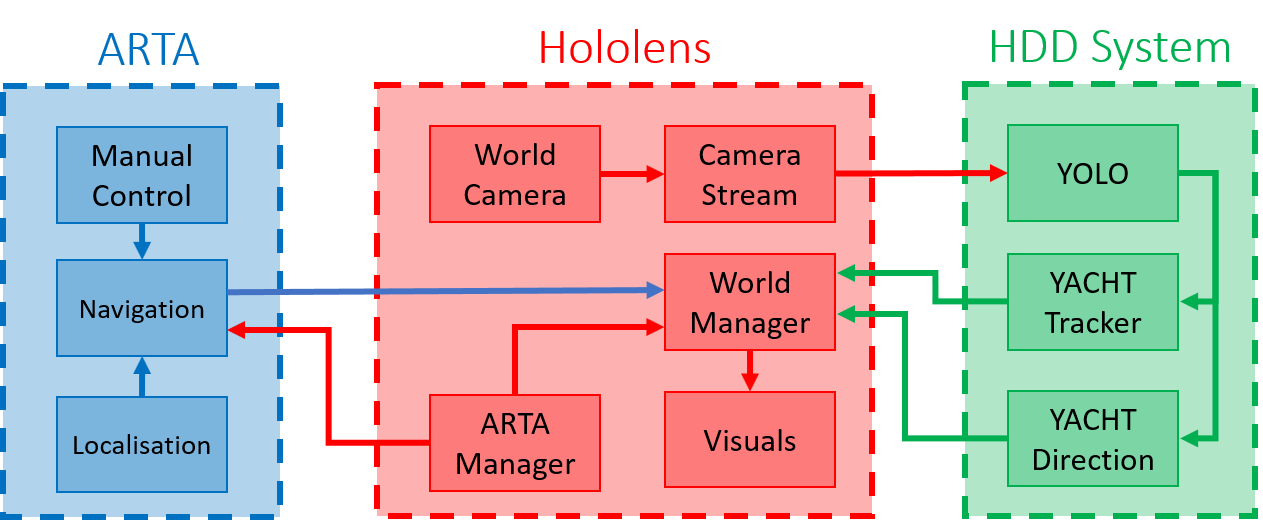
\includegraphics[width=1.0\linewidth]{img/chapter5_implementation/detailedSystemDiagram.png}
	\caption{System diagram detailing individual components}
	\label{fig:detailedHL}
\end{figure}

Figure \ref{fig:detailedHL} is a more detailed diagram of the high level system digram presented in Figure \ref{fig:simplifiedHL}. We show the communication between the three seperate devices, and how each node can be broken down into smaller nodes running specific computations. For the rest of this report, we represent the ARTA, Hololens and HDD system components with the colours blue, red and green respectively.

%\section{Hololens Video Camera Stream}
%For this project to begin, it was absolutely essential to stream the front-facing camera on the Hololens to another PC. Once it had been proven that this was possible, work on the rest of the project could begin. As such, the first month of the project was spent comparing different camera streaming methods. As mentioned in Section \ref{sec:videoStreaming}, we briefly spent some time attempting to use the HoloLensForCV library from Microsoft. However, after speaking with several members of the PRL, it was decided the best method would be to use the Unity application approach as a base.

\section{Human Detection \& Direction System}
In order to determine the direction people are walking in, it is necessary for the system to be able to detect humans. Only after detection is it possible to discern the motion of individuals, which can be achieved through object tracking and body pose estimation. Figure \ref{fig:detailedHDD} shows the breakdown of the HDD node into components responsible for these two tasks. This section is concerned with the implementation of the methods needed to perform the direction prediction, as well as how the system communicates between its nodes. 

\begin{figure}[ht]
	\centering
	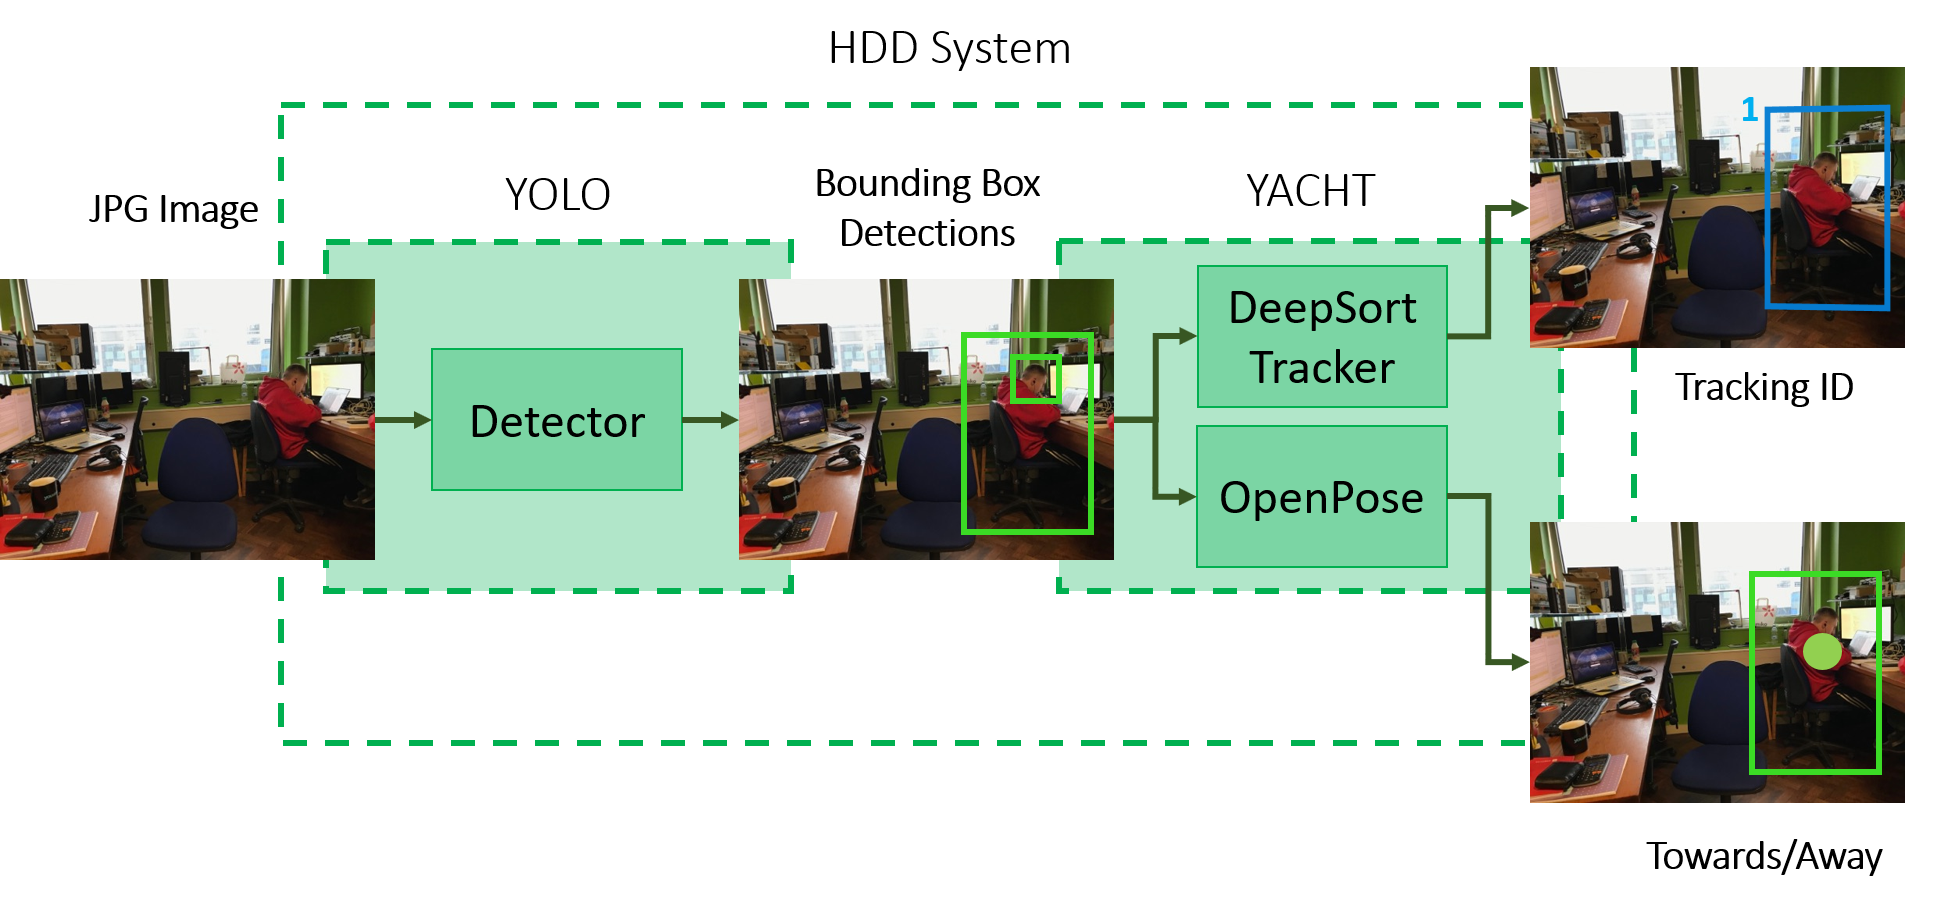
\includegraphics[width=1.0\linewidth]{img/chapter5_implementation/hddSystemDiagram.png}
	\caption{Individual nodes in HDD System}
	\label{fig:detailedHDD}
\end{figure}

We begin this section by listing the hardware requirements for the system. Due to the nature of the HDD, and its reliance on modern deep learning techniques, access to a modern GPU is essential. We refrain from trying to explain the step-by-step process to setup the hardware and software, and instead point the reader in the direction of an article\footnote{https://link.medium.com/xQ5w2FMXoX} which covers this topic.

\subsection{Hardware \& Software Dependencies}

\subsubsection{Hardware}
We implemented the HDD system on a desktop computer connected to the Imperial College network. Due to the real-time computer vision requirements of this project, the computer was chosen due to the GTX 1050Ti GPU with 4GB video RAM available on the system. The computer was also equipped with an Intel i7-2600 CPU and 8GB DDR3 RAM.

\subsubsection{Software}
We have refrained from posting all Python dependencies for the project and only mention the key ones. A complete listing is available in the appendix. The following software dependencies are required to run this project:
\begin{itemize}
	\item Ubuntu 16.04
	\item Python 2.7
	\item OpenCV 3.0
	\item ROS Kinetic
\end{itemize}

Due to the deep learning component of the project, the following software dependencies are essential:
\begin{itemize}
	\item Nvidia Graphics Drivers 
	\item CUDA 8.0 Toolkit
	\item cuDNN 6.0
	\item Darknet
	\item Tensorflow-GPU
	\item Caffe
\end{itemize}

\subsection{YOLO Object Detector}
As mentioned in Section \ref{sec:yolo}, we chose to use the YOLOv3 Tiny architecture and trained it on the CrowdHuman dataset. We begin this section by introducing the reader to \textbf{Darknet}, the neural network framework YOLO is implemented on, and how we integrated it into ROS. We also briefly explain how the network detects objects, and compare YOLOv3-tiny with the more memory intensive YOLOv3. We then guide the reader through the training process, and the analysis we did to validate the human detection improvements compared to pre-trained models.

\subsubsection{Darknet}
Darknet\footnote{https://pjreddie.com/darknet/} is an open source neural network framework written in C and CUDA which supports both CPU and GPU computation \cite{darknet13}. The source code for the framework is freely available on Github, and it can be used to train different neural network architectures in a manner similar to more conventional deep learning frameworks such as Tensorflow or Caffe.

\subsubsection{Darknet in ROS}
By definition, ROS is language-independent, although at the time of writing, three main libraries have been defined for ROS, making it possible to program ROS in Python, Lisp or C++. On the other hand, Darknet is implemented in C, due to the speed of compiled low-level languages in conjunction with CUDA. However, the Darknet framework is compiled into \textit{Shared Object (.so)} file, which is analogous to a Windows DLL. As such, it becomes possible to access the framework by writing wrappers around the compiled library file.

\paragraph{}Darknet has basic Python wrappers around the compiled library which convert Python datatypes into C and vice versa. However, the original wrappers for detection are written to run on images that are saved on disk. Darknet converts the saved images into a C data structure \code{IMAGE} and performs the detections. To integrate the framework into ROS, the node must be able to receive data from image topics with \code{CompressedImage} or raw \code{Image} messages.

\paragraph{}In ROS Python, the JPG or PNG images received from the \code{CompressedImage} message can be converted to numpy arrays which store the RGB values, without the need to be saved on disk. As such, we wrote Python wrappers for Darknet that allow the framework to support images in the form of numpy arrays as well as images saved on disk. The following listing defines the \code{IMAGE} data structure, and the conversion of an image numpy array to the Darknet format: \\



\begin{lstlisting}[language=Python, caption={Darknet IMAGE Python wrappers}]
# IMAGE: a C data structure used by Darknet
class IMAGE(Structure): 
	_fields_ = [("w", c_int),
				("h", c_int),
				("c", c_int),
				("data", POINTER(c_float))]
				
# Converts numpy array to Darknet IMAGE type
def nparray_to_image(img): 
	data = img.ctypes.data_as(POINTER(c_ubyte))
	image = ndarray_image(data, img.ctypes.shape, img.ctypes.strides)

	return image
\end{lstlisting}

Further Python wrappers were written for the detection and return of the image bounding box co-ordinates. We also created ROS messages for the bounding box detections, which allows the Darknet YOLO node to communicate with other nodes in the HDD system. The full code listing can be found in the Appendix \footnote{https://github.com/alaksana96/darknet-crowdhuman}\footnote{https://github.com/alaksana96/fyp\_yolo}.

\subsubsection{YOLO Detection Algorithm}
As researched in Section \ref{sec:backYOLO}, the algorithm divides an input image into an $S\times S$ grid. Each grid cell can predict one object, and a cell can predict a fixed number of bounding boxes $B$, which we visualize in Figure \ref{fig:yoloViz}. The predicted bounding box is chosen from the set of $B$ boxes with the highest box confidence score, which is a measure of how likely the box contains an object and how accurate the boundry box is. It also predicts the conditional class probability, which is the probability a detected object belongs to a certain class. 

\begin{figure}[ht]
	\begin{subfigure}[b]{.45\textwidth}
		\centering
		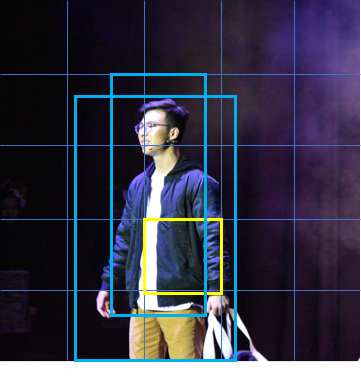
\includegraphics[width=1.0\linewidth]{img/chapter5_implementation/yoloAlgo1.png}
		\caption{A grid cell can make $B$ predictions, in this example $B=2$}
	\end{subfigure}%
	\hspace{\fill} 
	\begin{subfigure}[b]{.45\textwidth}
		\centering
		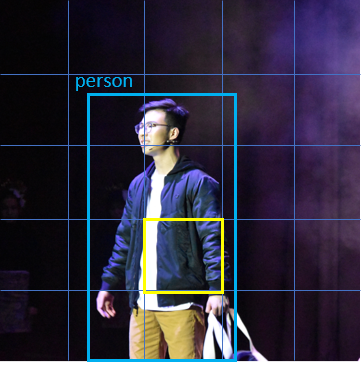
\includegraphics[width=1.0\linewidth]{img/chapter5_implementation/yoloAlgo.png}
		\caption{The bounding box with higher box confidence score is used}
	\end{subfigure}
	\vspace{-1\baselineskip}
	\begin{center}
		\caption{Visualization of YOLO person detection}
		\label{fig:yoloViz}
	\end{center}
	\vspace{-2\baselineskip}
\end{figure}

\subsubsection{YOLOv3 Tiny vs YOLOv3}
While testing out the different models, we noticed that the YOLOv3 model was consistently crashing and causing segmentation faults. On further investigation, we noticed that this was due to the network using up all 4GB of video memory available on the GPU. In comparison to its predecessors YOLO and YOLOv2, YOLOv3 is a much larger network which has 106 fully convolutional layers. Although it is far more accurate at predicting bounding boxes, it reduces the framerates that can be achieved on video. As such, we decided to use YOLOv3 Tiny, a shallower variant of the network that is suitable for real-time image detection. Although the tiny version is not as accurate, it is much lighter on memory, using less than 1GB video RAM, making it a suitable choice for this project.

\subsubsection{Training YOLOv3 Tiny}
\paragraph{CrowdHuman} The CrowdHuman dataset \cite{Shao} is a benchmark dataset to better evaluate detectors in crowd scenarios. The most important features of the dataset are the size, quality of the annotations and the diversity. Each image contains multiple people with varying degrees of occlusion, which allows for object detectors to better learn the representation of obscured people. 

\begin{figure}[ht]
	\centering
	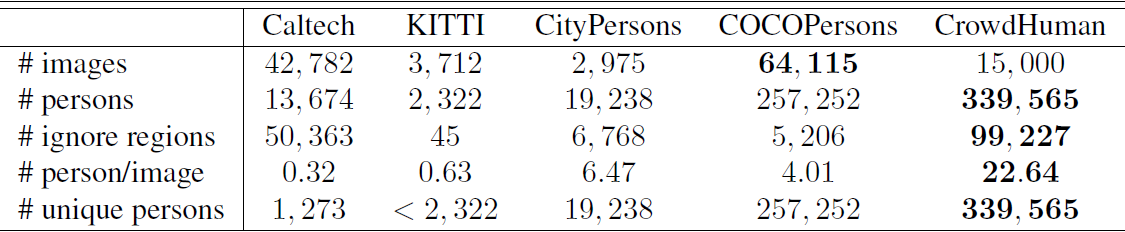
\includegraphics[width=0.8\linewidth]{img/chapter5_implementation/crowdHumanStats.png}
	\caption{A comparison of CrowdHuman to other person image datasets \cite{Shao}}
	\label{fig:crowdHumanStats}
\end{figure}

As can be seen from Figure \ref{fig:crowdHumanStats}, the dataset contains far more unique identities. By examining the dataset, we can see that it contains people in a wide array of situations, at varying distances with different body poses.

\paragraph{Annotations} The CrowdHuman dataset provides its annotations in the \code{.odtg} format, which is a variant of JSON. Each line in the annotation file corresponds to a JSON containing the image ID and the bounding boxes. The annotations include boxes for the \textit{visible box}, \textit{full body box} and \textit{head box}. For the purposes of this training, we chose to use the full body and head boxes only. We wanted the detector be able to learn to predict occluded individuals, and we also wanted to experiment with head pose estimation. Each bounding box is annotated as below, where \code{x,y} is the top-left corner of the bounding box. The \code{width} and \code{height} are also given in image co-ordinate pixels.

\paragraph{}\code{[x, y, width, height]}  

\paragraph{}On the other hand, to train YOLO on Darknet, the annotations must be given in a completely different format. The Darknet annotation format is as such:

\paragraph{}\code{<object-class> <x> <y> <width> <height>}

\paragraph{}Since Darknet accepts images of any size, it works with image units which are scaled relative to the size of the image. As such, all the values for the bounding boxes are between $0$ and $1$. Furthermore, the \code{x, y} values in the annotation are measured from the centre of the bounding box.  

\paragraph{Converting Annotations} To use the CrowdHuman images as a training set for the YOLOv3-tiny model, we had to write several scripts that converted the annotations to the Darknet format. We have included these scripts in the Appendix should the reader wish to convert the dataset themselves\footnote{https://github.com/alaksana96/darknet-crowdhuman/blob/master/README.md}.

\paragraph{Training Parameters} Before training, we set up the model configuration file to learn 2 classes, head and body, as well as to use batches of 32 divided into subdivision of 8 images. This limits the number of images loaded into memory at once to 8, to prevent running out of GPU memory. We also reduce the size of the training images to $416\times 416$ pixels, to further reduce the GPU usage. \\

\begin{lstlisting}[language=Mymatlab,caption={Training parameters}]
	batch=32 %Training parameters for YOLO Tiny
	subdivisions=8
	width=416
	height=416
	channels=3
	momentum=0.9
	decay=0.0005
\end{lstlisting}

These optimizations were done in order to maximize the amount of GPU memory used for training, without a sudden surge in usage causing a segmentation fault. Resizing the input training images allows the algorithm to divide the image into a $S\times S$ grid. Generally, the larger the height and width, the better the predictions, since the image can be divided into more grid cells. This is a trade-off we had to make in order to be able to train the network on a mid-range GPU.

\paragraph{Training Process} We left the model to train overnight, creating backups of the weights every 1000 iterations. The following day, after reaching 30,000 iterations, we decided to stop training the network. The average loss error and total loss had stopped decreasing for several hours, and was hovering around $29.134$. We reasoned that the network had reached a minima, and further training would be redundant, since it would overfit the dataset. The final weights are available in the file \code{yolov3-tiny-crowdhuman.backup} .

\subsubsection{Evaluating Trained Model}
\paragraph{Hololens Videos} As mentioned in Section \ref{sec:backYOLO}, we recorded several test videos using the Microsofto Hololens. These videos were capture in various locations on the Imperial College campus. A common area where lots of people frequent is the Sherfield walkway. As seen in Figure \ref{fig:yoloSherfield}, this was an ideal place to capture a video since it features a lot of people walking around in different directions. We captured several more videos outside the EEE building and inside the 5th floor ICRS lab. 

\begin{figure}[ht]
	\centering
	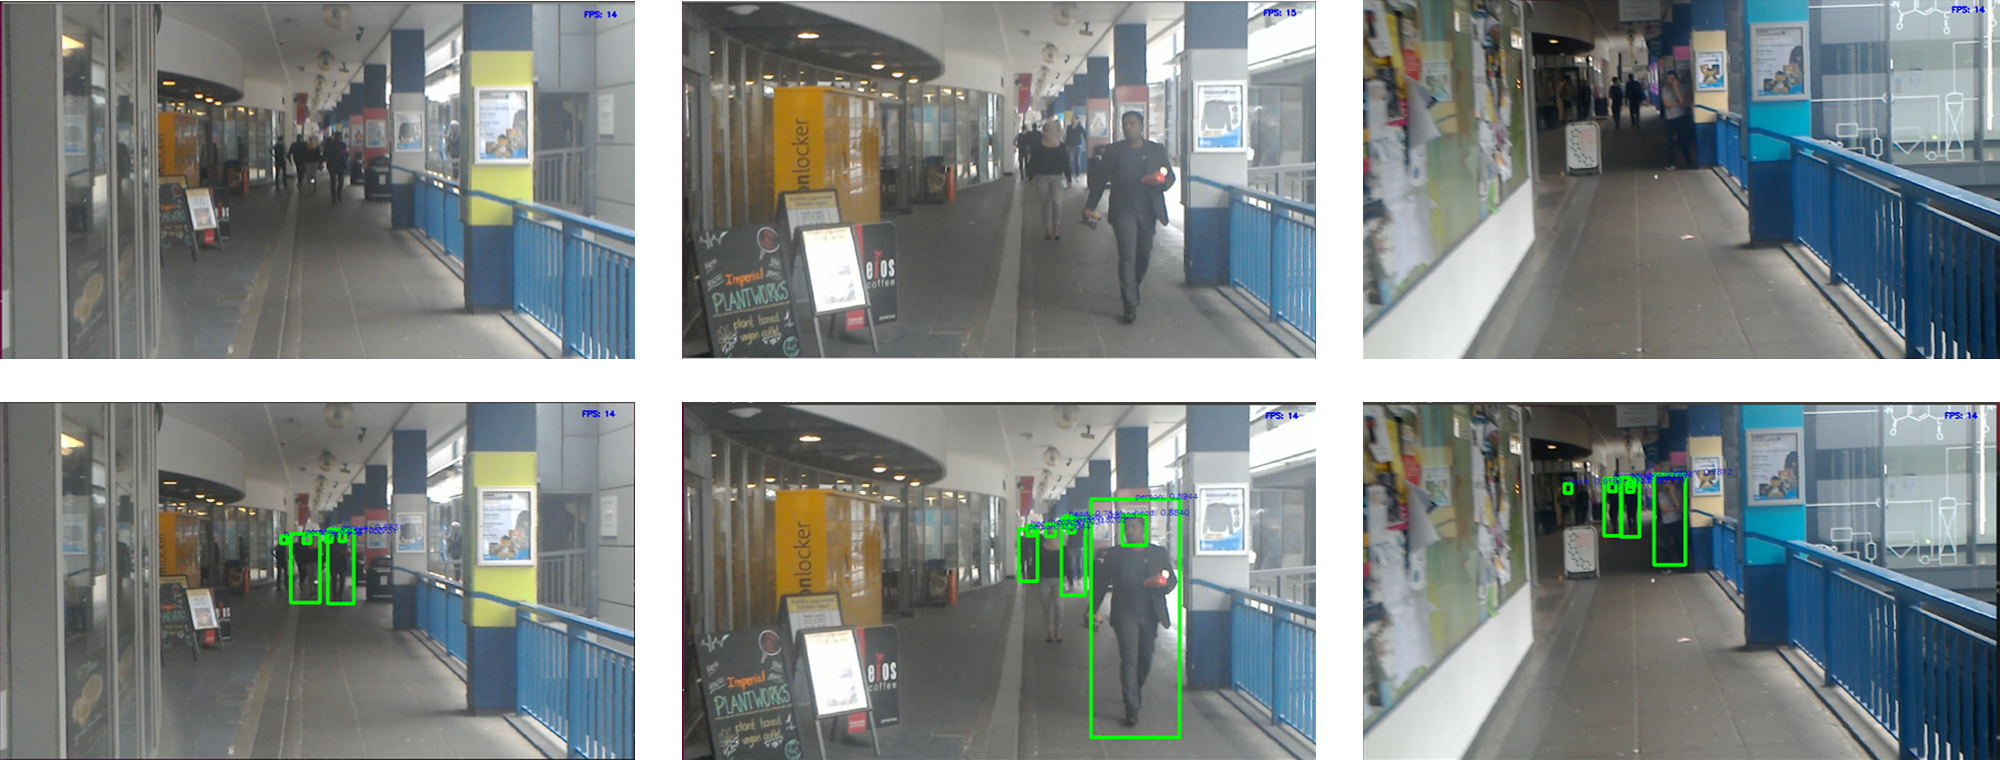
\includegraphics[width=0.95\linewidth]{img/chapter5_implementation/yoloWalkwayMultiple.png}
	\caption{Evaluating the model on Sherfield Walkway test video}
	\label{fig:yoloSherfield}
\end{figure}

\paragraph{} The videos from the Hololens were captured whilst a person was walking with the device, to best emulate a PWU in a wheelchair navigating through populated areas. We noticed an improvement in the number and accuracy of the detected bounding boxes compared with the pre-trained COCO models provided by Darknet. The most significant improvement to the model was the ability to detect objects at different ranges, as shown in Figure \ref{fig:yoloRange}. 

\begin{figure}[ht]
	\centering
	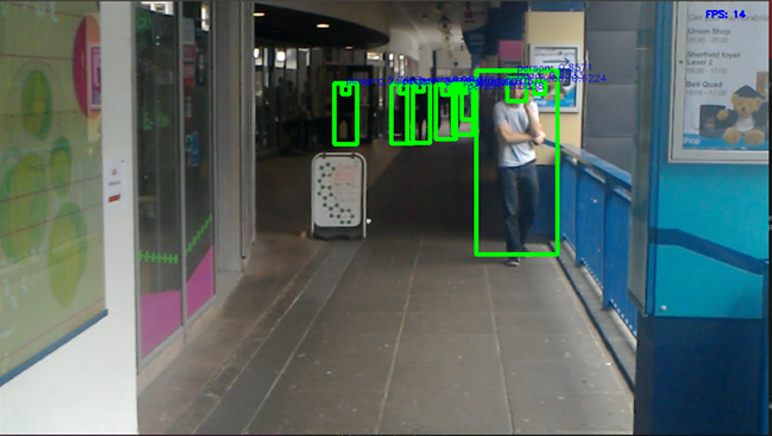
\includegraphics[width=0.8\linewidth]{img/chapter5_implementation/yoloWalkway.png}
	\caption{Trained model detects people and heads at different ranges}
	\label{fig:yoloRange}
\end{figure}

\subsubsection{ROS Node} \label{sec:nodeYOLO}
The Python wrappers for Darknet allow us to access the detection and image conversion functionality of the framework. To fully integrate the framework as a ROS node, we must follow the standard ROS procedures for creating a new ROS package. As such, we have created a package\footnote{https://github.com/alaksana96/fyp\_yolo} that runs Darknet and YOLO that can be downloaded and run seamlessly with ROS.

\paragraph{ROS Topics} The ROS node subscribes to the \code{/image\_transport/compressed} and expects to receive images in the compressed JPG format. This is because the Hololens captures video frames and encodes it to reduce the usage on the network bandwidth. These images are converted to numpy arrays which are further converted to Darknet \code{IMAGE} types for detection. 

\paragraph{} Darknet produces bounding box co-ordinates and class probabilities for each detection in an image. For every received frame, the node publishes the original image and a list of associated bounding boxes. The bounding box message contains the following information: \\

\begin{lstlisting}[language=Mymatlab,caption={BoundingBox.msg},label={bbmsg}]
string Class
float64 probability
int64 xmin % Top Left Corner
int64 ymin
int64 xmax % Bottom Right Corner
int64 ymax
\end{lstlisting}

\subsection{YACHT Package}
The major contribution of this project is in the form of the Yet Another Crowd Human Tracker package for ROS. This package utilizes the Deep SORT algorithm and OpenPose body pose estimation framework to attempt to determine the direction of individuals.


\paragraph{ROS Communication} As seen in Section \ref{sec:nodeYOLO}, the YOLO object detector node publishes a topic which contains the image and associated bounding boxes. Figure \ref{fig:detailedHL} shows that both YACHT nodes subscribe to the same output topic. The reason we decided to include the original image in the message and not just the bounding boxes is so that we can be sure the bounding boxes were detected for that frame, without having to subscribe to two seperate topics and comparing timestamps on individiual messages.

\subsection{YACHT: Tracker}
As explained in Section \ref{sec:YACHT}, the YACHT tracker depends on the Deep SORT algorithm \cite{Wojke2018}. Using the detections produced by the YOLO node, we assign IDs and match them across video frames to produce a track. These tracking IDs are then sent to the HoloLens for visualizaiton.


\subsubsection{Deep SORT} 

\paragraph{Modifications} We have modified\footnote{https://github.com/alaksana96/deep\_sort} Nicolai Wojke's original implementation of Deep SORT to run on Tensorflow-GPU. In the original, as the number of detections increased, so does the delay in tracking. This issue is more prevalent when tested on the MOT dataset, which has a large number of objects in each frame. Figure \ref{fig:deepSortCPU} visualizes the delay on the MOT16-06 video. We can see that the algorithm is operating at a very low FPS, causing it to be delayed in time. 

\begin{figure}[ht]
	\begin{subfigure}[b]{.45\textwidth}
		\centering
		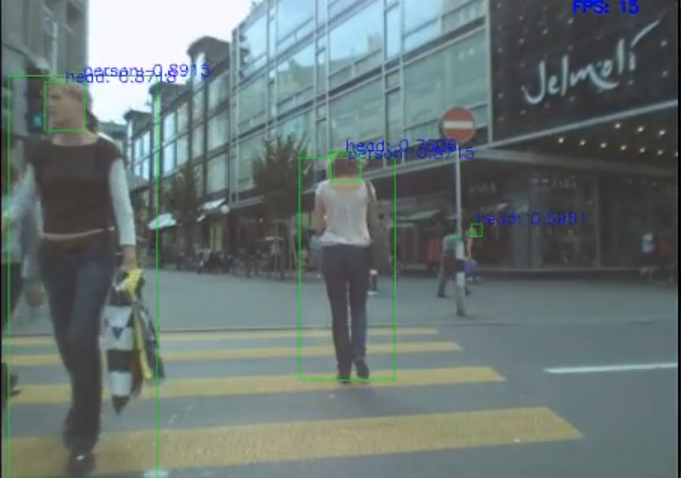
\includegraphics[width=1.0\linewidth]{img/chapter5_implementation/deepSortCPU.png}
		\caption{Output of YOLO. The image frame and bounding boxes are fed to Deep SORT}
	\end{subfigure}%
	\hspace{\fill} 
	\begin{subfigure}[b]{.45\textwidth}
		\centering
		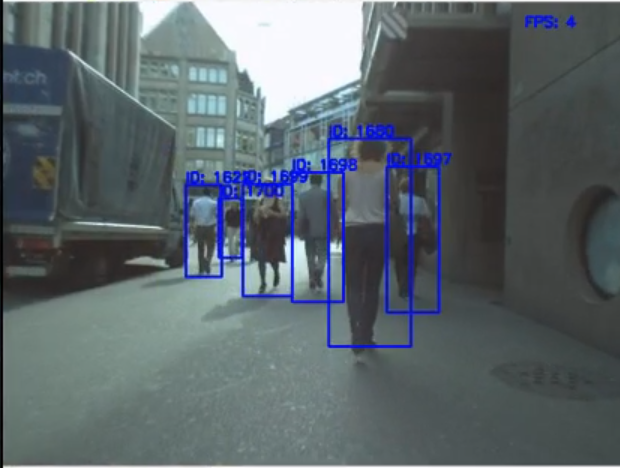
\includegraphics[width=0.935\linewidth]{img/chapter5_implementation/deepSortCPU1.png}
		\caption{Deep SORT is several frames behind since it runs at 4 FPS}
	\end{subfigure}
	\vspace{-1\baselineskip}
	\begin{center}
		\caption{Visualization of delay on CPU bound Deep SORT}
		\label{fig:deepSortCPU}
	\end{center}
\end{figure}


\paragraph{Deep Association Metric} Through code profiling, we noticed that the program was spending a lot of time in the generation of feature vectors. Upon inspection, we noticed that this process was run on a CPU bound version of Tensorflow. The \code{ImageEncoder} class uses a pre-trained deep network that generates the feature vectors for each bounding box. By using Tensorflow-gpu, we were able to run the network on system GPU, removing the delay. \\

\begin{lstlisting}[language=Python, caption={Deep SORT Tensorflow GPU modifications}]
class ImageEncoder(object):

	def __init__(self, checkpoint_filename, input_name="images",
				 output_name="features"):
				 
        # Tensorflow-GPU
        gpu_options = tf.GPUOptions(per_process_gpu_memory_fraction = 0.2)
        self.session = tf.Session(config=tf.ConfigProto(gpu_options=gpu_options))
\end{lstlisting}

%The tracker crops the image and generates feature vectors for the detection. The vectors are then compared with the history of feature vectors associated with each tracker.

\paragraph{Trackers \& Tracking} For each detection, we generate a feature vector using the image pixels within the bounding box. A matching cascade with Nearest Neighbour metric is used to best match the detection with existing confirmed tracks. Some detections will not get matched since the distance to confirmed tracks is above the \code{matching\ threshold}. The algorithm then attempts to match the detections to unconfirmed tracks using a simple Intersection-over-Union metric. These are newly created tracks that have existed for less than the last $n$ frames. If the detection is still unmatched, the algorithm creates a new tracker for the detection and adds it to the pool of unconfirmed tracks.

\begin{figure}[ht]
	\centering
	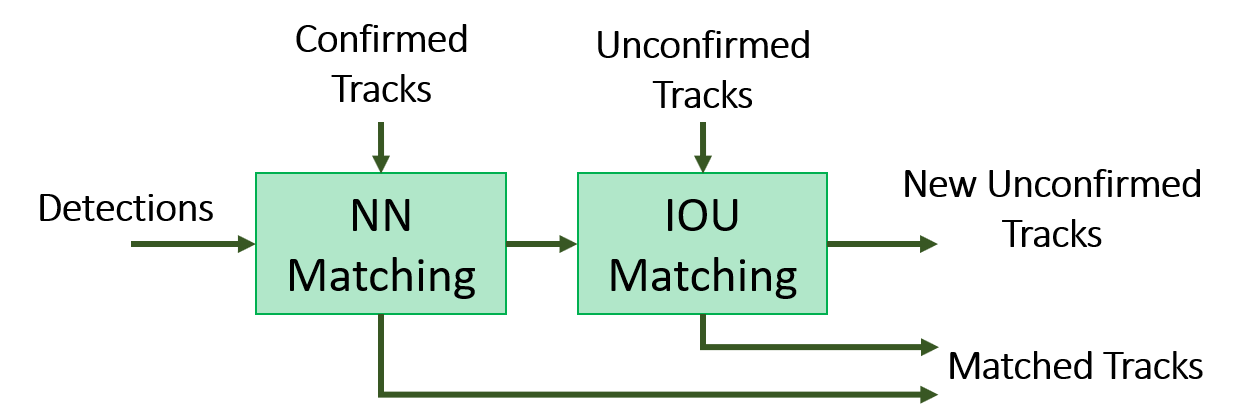
\includegraphics[width=0.8\linewidth]{img/chapter5_implementation/deepSortMatching.png}
	\caption{Deep SORT matching visualized}
	\label{fig:deepSortMatch}
\end{figure}

Any pre-existing tracks which are not matched are checked. If the number of frames since the previous match is greater than the \code{max\_age} parameter, the track is considered dead and is deleted. This is done so as to prevent the number of tracks from growing unboundedly. A Kalman filter is used to update the bounding box states of each track, as well as the time since the last update.
 
\subsubsection{Linear Extrapolation}
We experimented with linear extrapolation across frames as a way of infering the direction travelled by the detection. As the project progressed, we encountered issues with this method, as explained in Section \ref{sec:objecTrackingDirection}. By searching for alternative methods, it was found that the depth camera on the Hololens can determine the distance between the PWU and an object relatively accurately. As such, we abandoned the pure computer vision approach in favour of using the Hololens.

\subsubsection{ROS Topic} The decision to use the Hololens depth cameras as a way of determining distance prompted the need for ROS messages to be sent to the device. As seen in Figure \ref{fig:detailedHDD}, the  tracker node publishes the bounding box and tracker ID to the Hololens. The \code{BoundingBox} data structure is defined in Listing \ref{bbmsg}, and is the same bounding boxes generated by the YOLO detector.

\begin{lstlisting}[language=Mymatlab,caption={BoundingBoxID.msg}]
BoundingBox boundingBox
int64       id
\end{lstlisting}

\subsection{YACHT: Direction}
The second node in the YACHT package is the direction node, which uses the OpenPose framework to determine if a person is facing the camera or not. Earlier in Section \ref{des:YACHTBody}, we outlined the problem of not being able to determine the distance to an object with a regular pinhole camera model. We initally wanted to be able to determine the distance using only a video stream and computer vision techniques. However, we quickly realized that this was beyond the scope of the project, and decided to use the depth cameras on the Hololens.

\paragraph{} This section outlines the installation and setup of the OpenPose network \cite{Shao}. We also explain how we use the keypoint detections to determine whether an individual is facing the PWU or not. Furthermore, we also explain how the bottom-up approach of OpenPose differs from the top-down approach that may have been more suitable, and the reasons for our implementation choices.

\subsubsection{OpenPose}
OpenPose is developed and maintained by the Carnegie Mellon University Perceptual Computing Lab. The implementation is made available on Github\footnote{https://github.com/CMU-Perceptual-Computing-Lab/openpose} to encourage body pose estimation research.

\paragraph{Installation \& Setup} The OpenPose library runs on a modified version of the convolutional neural network framework Caffe \cite{Jia}. The library is well documented, and provides its own instructions on how to setup the library. We direct the reader to the OpenPose Github repository if they wish to install the library themselves.

\paragraph{Model} As stated in Section \ref{des:body_25}, we use the \code{BODY\_25} keypoint estimation model for this project. The documentation states that this model is the fastest when it comes to real-time application, compared to the \code{MPI\_4} or \code{COCO} models. We also reduce the network resolution to $176\times 176$ to reduce the GPU usage and speed up the keypoint estimation. However, this reduces the accuracy of the detections, as discussed in this section.

\subsubsection{KeyPoint Estimation} \label{sec:bottomUp} 
Due to the bottom-up approach used by OpenPose, the network predicts keypoints for individual body parts across the whole image. Through our testing on the MOT dataset, we noticed several points:

\begin{itemize}
	\item The model is good at detecting keypoints of people close to the camera.
	\item People who are smaller and further away are not always detected.
	\item When people are close together or overlap, the keypoint estimation has difficulty differentiating between people.
	\item The more people in the image, the more network slows down and begins to lag behind the source video.
\end{itemize}

\begin{figure}[ht]
	\begin{subfigure}[b]{.32\textwidth}
		\centering
		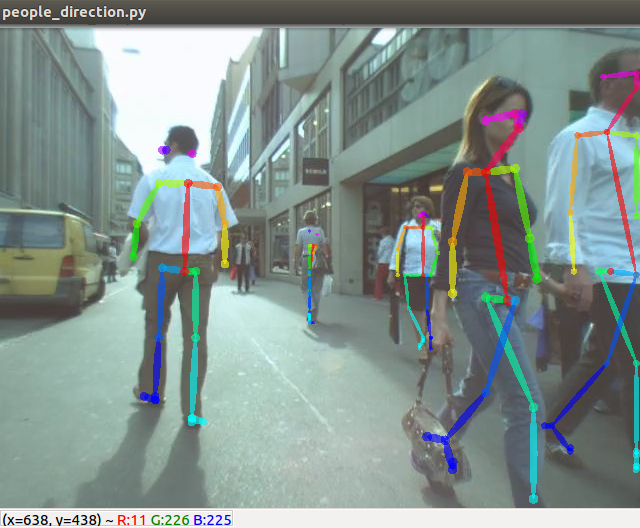
\includegraphics[width=1.0\linewidth]{img/chapter5_implementation/openposeKP.png}
		\caption{People close-up}
	\end{subfigure}%
	\hspace{\fill} 
	\begin{subfigure}[b]{.32\textwidth}
		\centering
		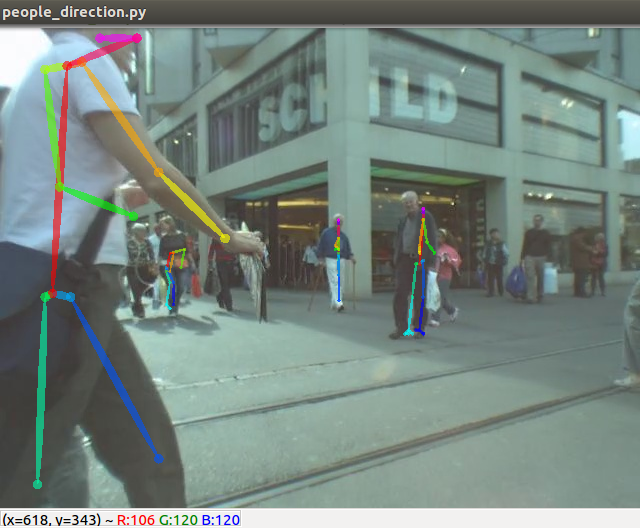
\includegraphics[width=1.0\linewidth]{img/chapter5_implementation/openposeKP1.png}
		\caption{People at different scales}
	\end{subfigure}
	\hspace{\fill} 
	\begin{subfigure}[b]{.32\textwidth}
		\centering
		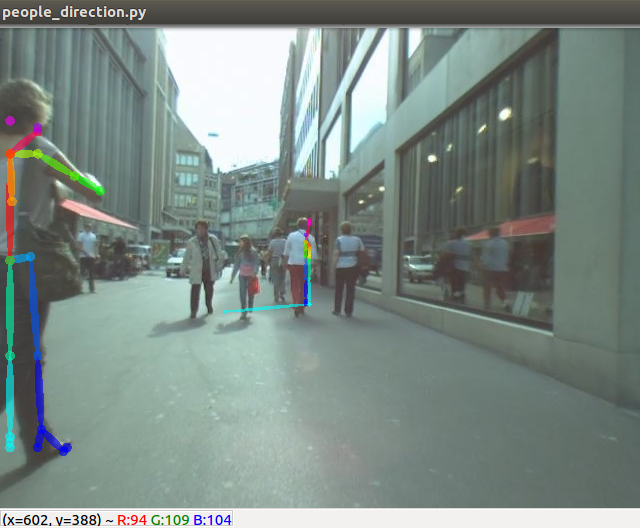
\includegraphics[width=1.0\linewidth]{img/chapter5_implementation/openposeKP2.png}
		\caption{People close together}
	\end{subfigure}
	\vspace{-1\baselineskip}
	\begin{center}
		\caption{Comparison of keypoint estimation at different scales}
		\label{fig:openposeKP}
	\end{center}
		\vspace{-1.5\baselineskip}
\end{figure}

We highlight the issues in Figure \ref{fig:openposeKP}. The reason for the decrease in accuracy on people further away is due to the network resolution being lowered. Using a higher resolution allows us to detect people further away, but the delay between the arrival of the frame and the detection is more than 0.5 seconds. As such, to achieve real-time operation, we chose to use a lower network resolution.

\subsubsection{Defining Direction}
By comparing the relative positions of certain keypoints, we can determine if a person is facing towards the camera or if they are walking away. This information is important, since it will allow for better visualization of where a person is walking, since people tend to walk in the direction they are facing. This also partially solves the direction problem brought up in Section \ref{sec:objecTrackingDirection}.

\begin{figure}[ht]
	\begin{subfigure}[b]{.32\textwidth}
		\centering
		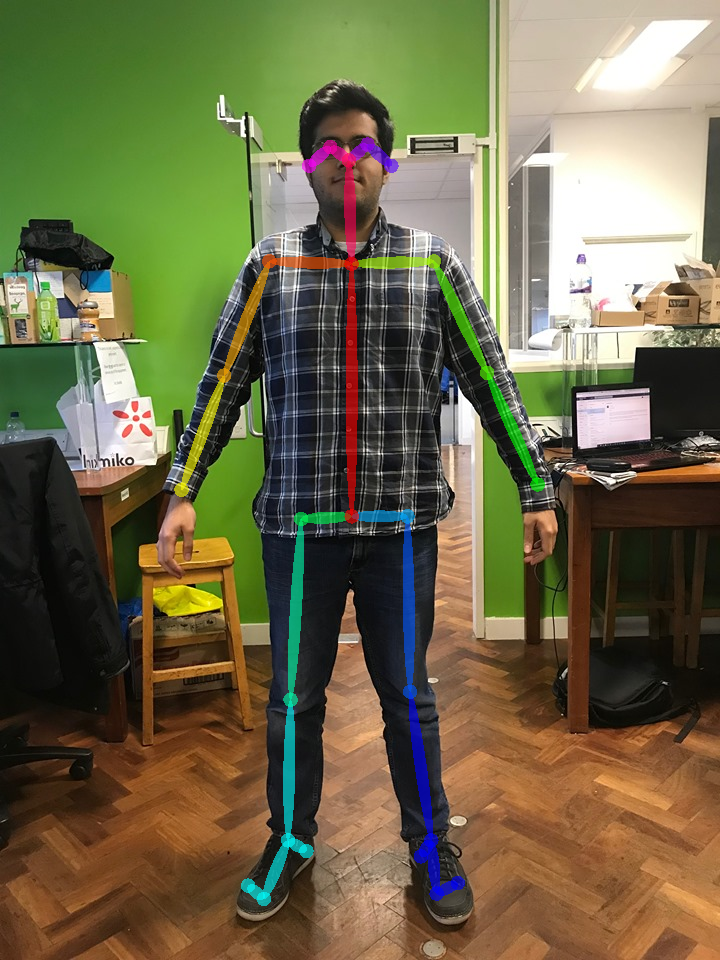
\includegraphics[width=1.0\linewidth]{img/chapter5_implementation/shreyFront.png}
		\caption{Frontal View}
	\end{subfigure}%
	\hspace{\fill} 
	\begin{subfigure}[b]{.32\textwidth}
		\centering
		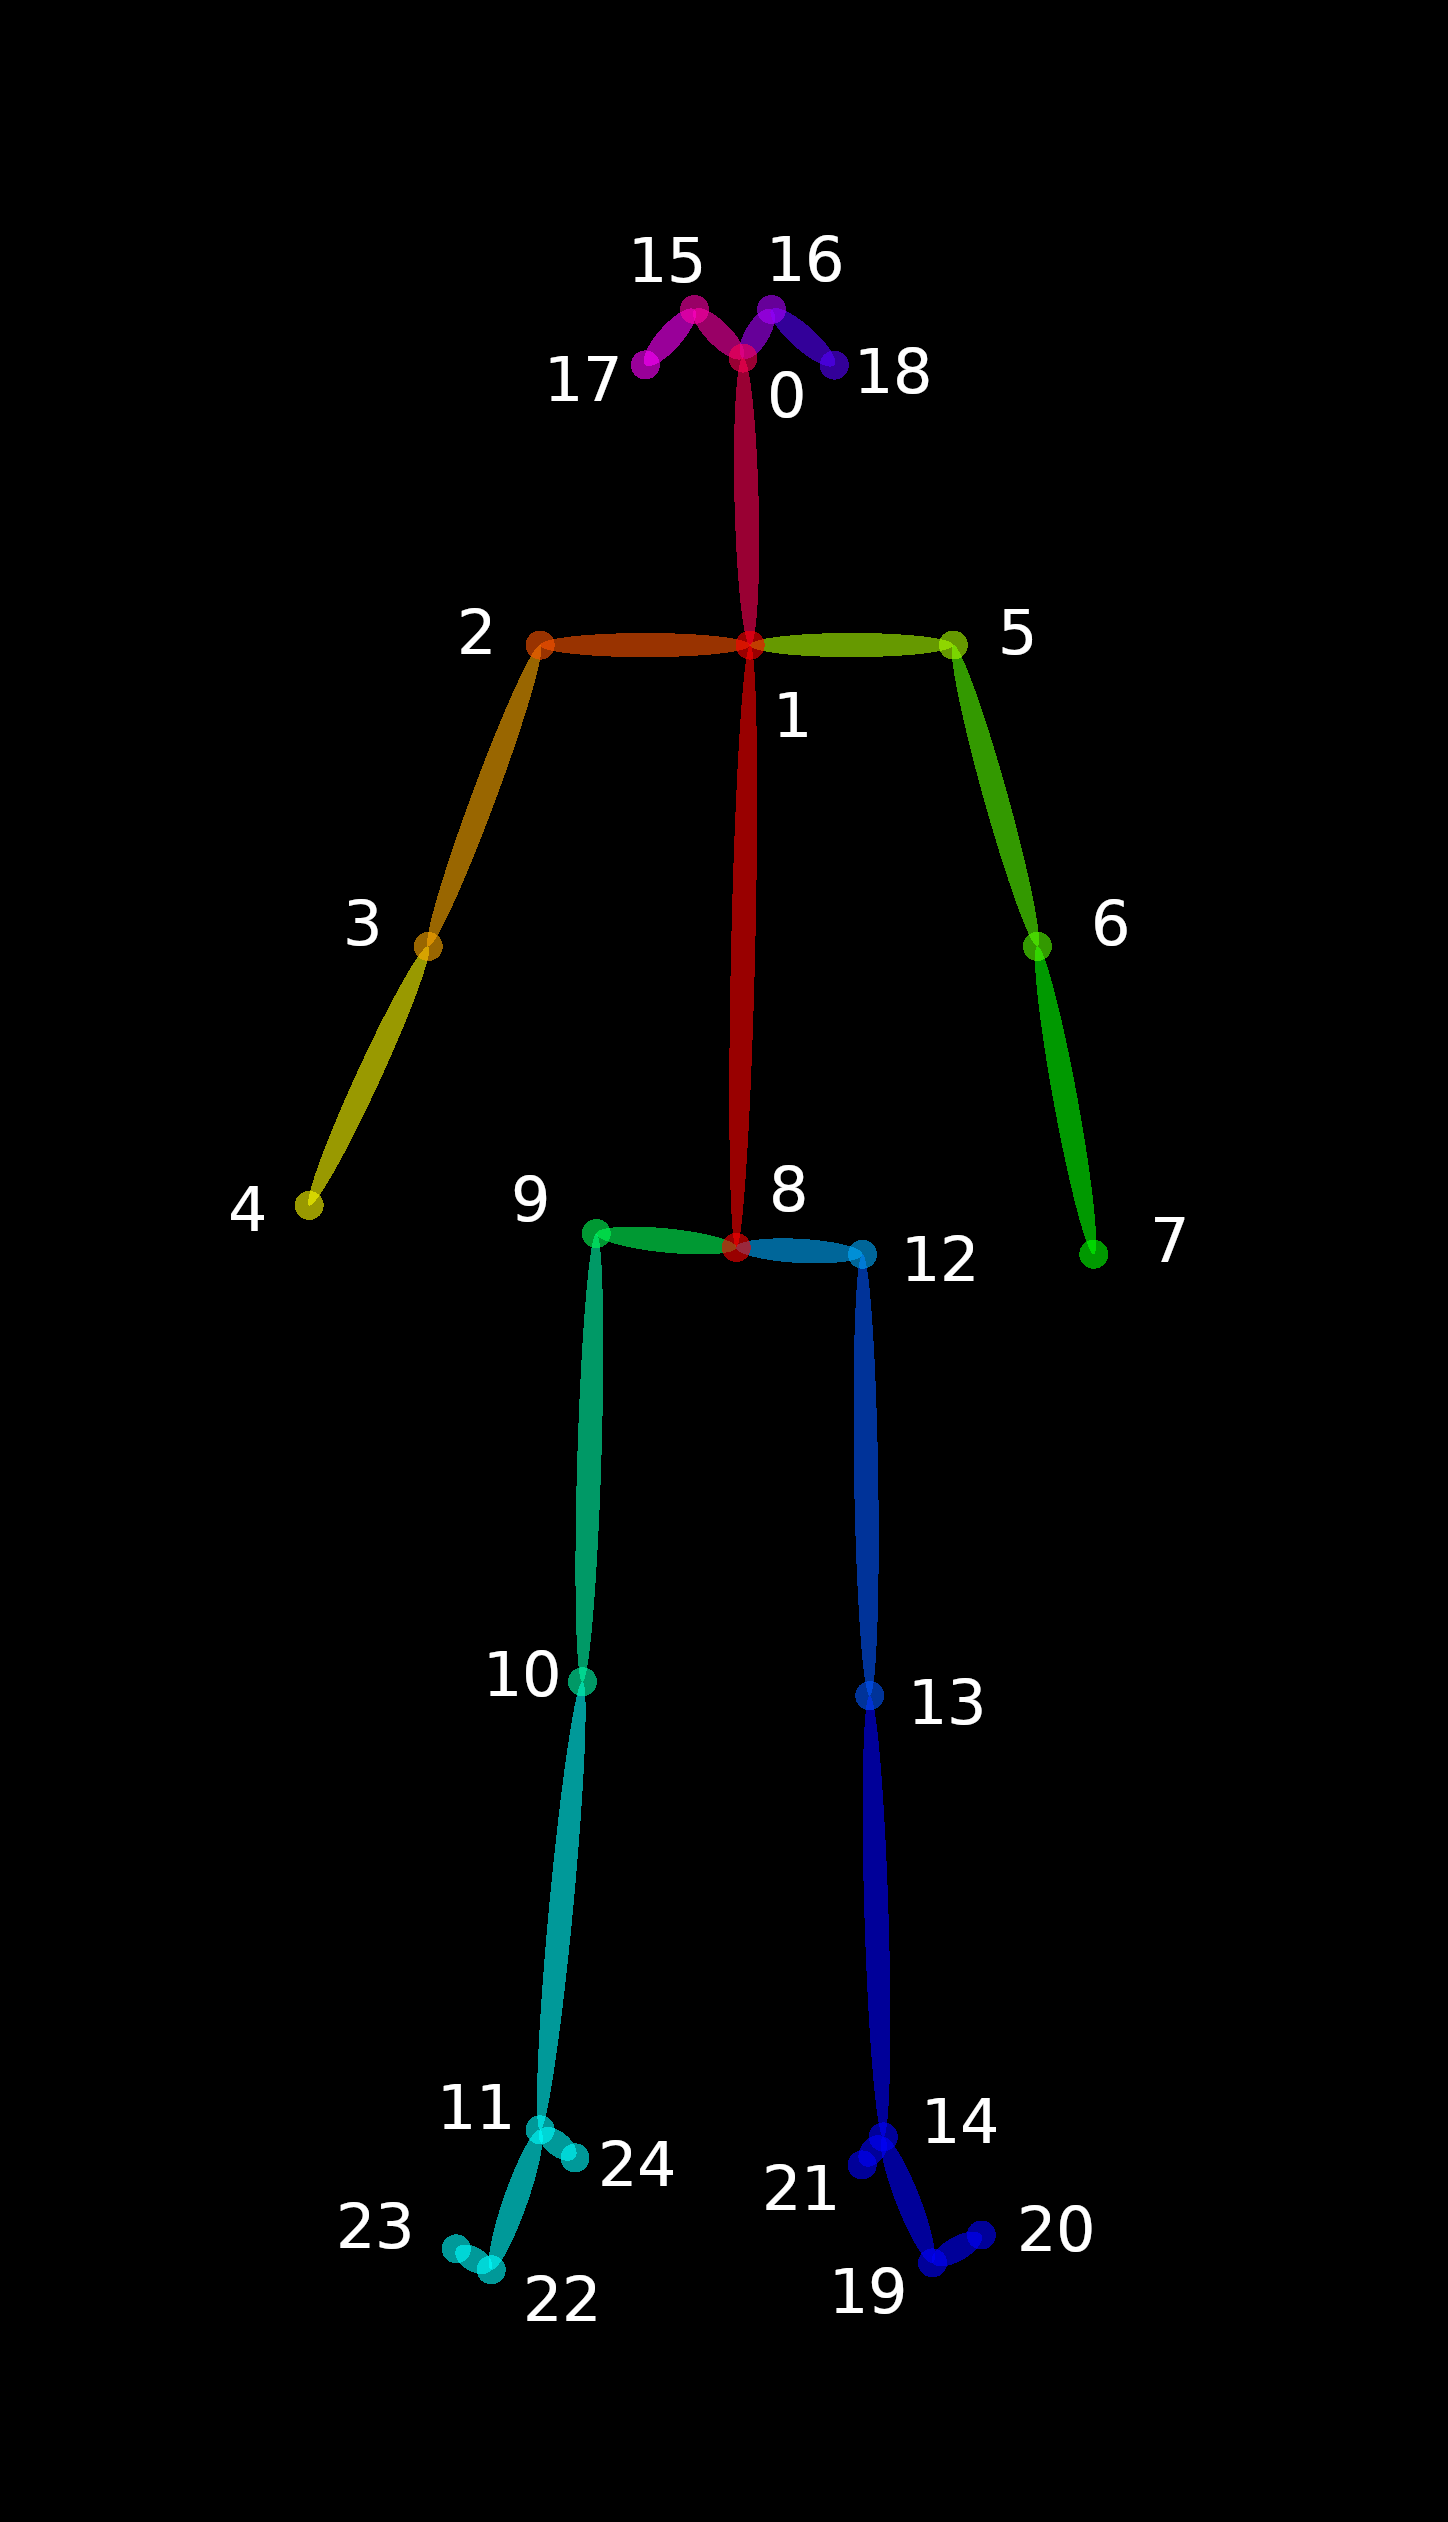
\includegraphics[width=0.765\linewidth]{img/chapter5_implementation/keypoints_pose_25.png}
		\caption{Keypoint References}
	\end{subfigure}
	\hspace{\fill} 
	\begin{subfigure}[b]{.32\textwidth}
		\centering
		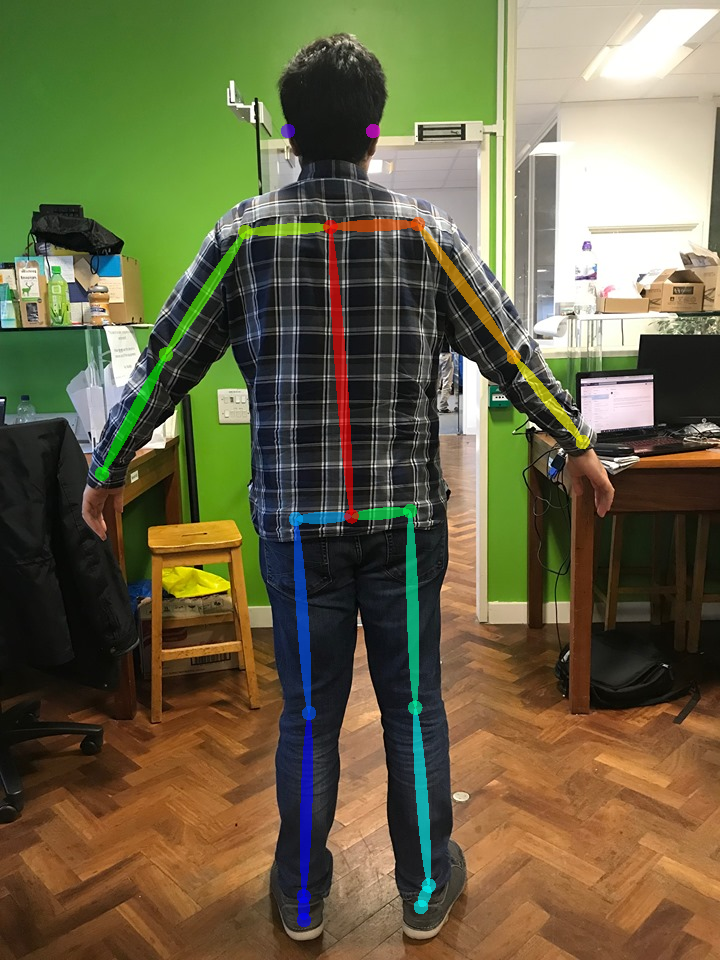
\includegraphics[width=1.0\linewidth]{img/chapter5_implementation/shreyBack.png}
		\caption{Back View}
	\end{subfigure}
	\vspace{-1\baselineskip}
	\begin{center}
		\caption{Body keypoint estimation of different views}
		\label{fig:keypointShrey}
	\end{center}
	\vspace{-2\baselineskip}
\end{figure}

\paragraph{Method} Pixels are measured from the top left corner of the image, with the x-axis extending horizontally to the right and the y-axis extending downwards. Figure \ref{fig:keypointShrey}.b shows the keypoint references for the body. The model is able to differentiate between the left and right limbs on a person. Figure \ref{fig:keypointShrey}.(a,c) show a full frontal and back keypoint detection on a person in the ideal detection position. 

\begin{table}[ht]
	\centering
	\begin{tabular}{|l|l|}
		\hline
		Body Part  & Key Points \\ \hline
		Right Arm  & 2, 3, 4    \\ \hline
		Left Arm   & 5, 6, 7    \\ \hline
		Head/Spine & 0, 1, 8    \\ \hline
	\end{tabular}
	\caption{Significant keypoints for direction}
	\label{tab:keypoints}
\end{table}

We can use the ability to differentiate between the left and right arms to determine if a person is facing the camera. Table \ref{tab:keypoints} presents the keypoints for the relevant bodyparts. If the image co-ordinates of the left shoulder is further along the x-axis than the right shoulder, we can predict the direction as facing towards the camera. From testing, we know this simple method works most of the time. However, problems arise when a person is standing perpendicular to the camera. OpenPose has trouble detecting the torso and predicting the positions of the limbs, and it becomes difficult to decide if they are facing left or right.

\subsubsection{Implementation \& Detection Matching}
As mentioned in Section \ref{sec:bottomUp}, OpenPose uses a bottom-up approach by detecting individual body parts across the whole image. We need to match the OpenPose keypoint predictions with existing bounding boxes from YOLO, since these are assigned track IDs by the tracker node. This is done in Listing \ref{lst:matchDetPose} \\

\begin{lstlisting}[language=Python, caption={Direction and Detection Matching}, label={lst:matchDetPose}]
def matchDetectionAndPose(self, detections, poses):
    for pose in poses:
        # Check torso, right/left shoulder
        torso, rshoulder, lshoulder = pose[1], pose[2], pose[5]

        for bbox in detections:
            if( self.withinBB(bbox, torso[0], torso[1]) or
                self.withinBB(bbox, rshoulder[0], rshoulder[1]) or
                self.withinBB(bbox, lshoulder[0], lshoulder[1])):
   
                if(rshoulder[0] > lshoulder[0]):
                    directionTowardsCamera = False
                else:
                    directionTowardsCamera = True

                publishDetectionDirection() 
                break # Once matched, move onto next pose 
\end{lstlisting}

\subsubsection{ROS Topic}
The direction node publishes the bounding box and direction to the Hololens. The \code{BoundingBox} data structure is defined in Listing \ref{bbmsg}, and is the same bounding boxes generated by the YOLO detector. \\

\begin{lstlisting}[language=Mymatlab,caption={BoundingBoxDirection.msg}]
BoundingBox boundingBox
bool        directionTowardsCamera
\end{lstlisting}

\newpage
\section{Hololens Unity Application}

\begin{figure}[ht]
	\centering
	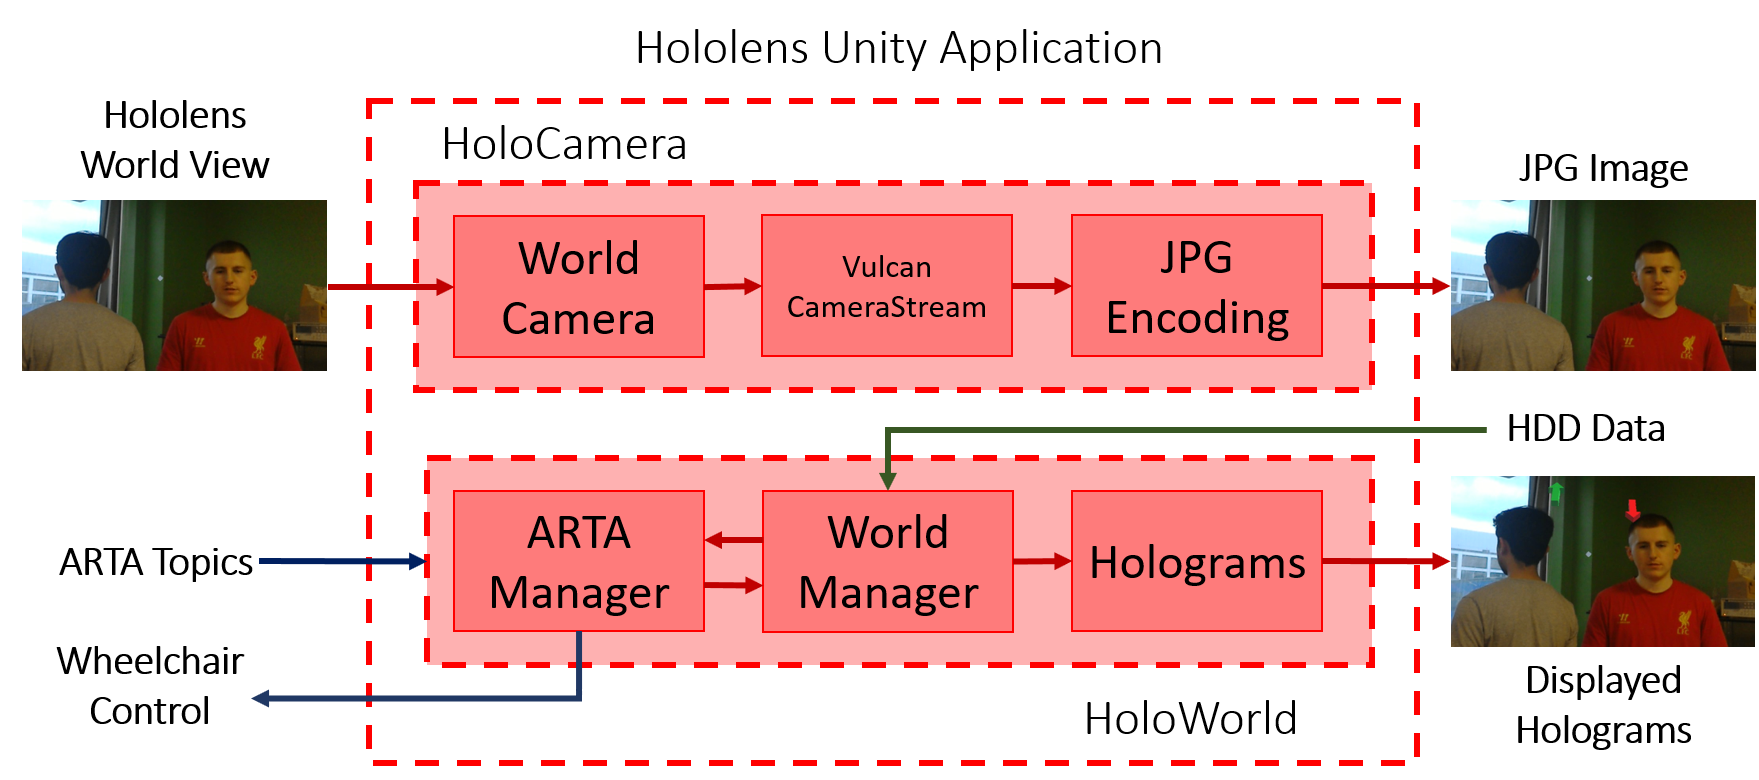
\includegraphics[width=1.0\linewidth]{img/chapter5_implementation/hololensSystemDiagram.png}
	\caption{Unity application running on the Hololens}
	\label{fig:detailedHololens}
\end{figure}
